\doublespacing
\setlength{\parindent}{1cm}

To understand Convolutional Neural Networks, we have to understand the following foundational ideas:

\begin{itemize}
  \item Convolution
  \item Pooling
  \item Jargon: padding, stride, filter, etc
\end{itemize}

In computer vision, we have used diverse techniques in the past on images to do object detection and image classification. One major problem with computer vision problems is that the input data can get really big. Suppose an image is of the size 68 X 68 X 3. The input feature dimension then becomes 12,288. This will be even bigger if we have larger images (say, of size 720 X 720 X 3). Now, if we feed this big input to a neural network, the number of parameters will swell up to a very large number (depending on the number of hidden layers and hidden units). This will result in more computational and memory requirements – not something most of us can deal with. \par

We begin by looking at edge detection as a simple example. The early layers of a neural network detect edges from an image. Deeper layers might be able to detect the cause of the objects and even more deeper layers might detect the cause of complete objects (like a person’s face). \par

\textbf{Edge Detection Problem}

In this section, we will focus on how the edges can be detected from an image. Suppose we are given the figure below:

\begin{figure}
  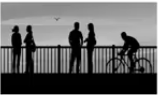
\includegraphics{edge-fig-1.png}
\end{figure}
